\documentclass[a4paper,nobind]{ociamthesis}  % no extra pages
% \documentclass[a4paper,twoside,hidelinks]{ociamthesis}  % uncomment lines 99 and 100 in ociamthesis.cls
% \documentclass[a4paper]{ociamthesis}  % one-sided binding


%%% PACKAGES %%%
\usepackage{tikz}
\usepackage{float}
\usepackage{lipsum}
\usepackage{xpatch}
\usepackage{custom}
\usepackage{subfig}
\usepackage{physics}
\usepackage{amsmath}
\usepackage{graphicx}
\usepackage{quantikz}
\usepackage{listings}
\usepackage{standalone}
\usepackage{circuitikz}
\usepackage{blochsphere}


%%% DRAFT VERSION %%%
\fancyfoot[C]{\emph{DRAFT Printed on \today}}  % draft in footer


%%% CORRECTIONS %%%
\correctionstrue  % comment out to remove corrections in blue
% \mccorrect{blah}  % word corrections
% \begin{mccorrection} ... \end{mccorrection}  % paragraph corrections


%%% GRAPHICS %%%
\graphicspath{{figures/}}


%%% BIBLIOGRAPHY %%%
\bibliographystyle{ref_style}

% uncomment for equations numbered per section rather than per chapter
% \numberwithin{equation}{subsection}


%%% TITLE PAGE %%%
\title{Diagrammatic Design of Ansätze for Quantum Chemistry}
\author{Ayman El Amrani}
\college{St. John's College}
\degree{Honour School of Chemistry}
\degreedate{Part II 2024}


%%% MACROS %%%
\renewcommand{\th}{\textsuperscript{th}}  % text superscripts
\newcommand{\nd}{\textsuperscript{nd}}
\renewcommand{\st}{\textsuperscript{st}}
\newcommand{\rd}{\textsuperscript{rd}}


%%% ========== BEGIN DOCUMENT ========== %%%
\begin{document}

%%% LINE SPACING CONFIG %%%
% \setlength{\textbaselineskip}{26pt}  % official line spacing
\setlength{\textbaselineskip}{22pt}  % official line spacing
\setlength{\frontmatterbaselineskip}{17pt plus1pt minus1pt} % roman pages
\setlength{\baselineskip}{\textbaselineskip}

%%% SECTION NUMBERING DEPTH CONFIG %%%
\setcounter{secnumdepth}{1}  % level that is numbered
\setcounter{tocdepth}{1}  % level that appears in table of contents


%%% ========== ROMAN PAGES ========== %%%
\begin{romanpages}
\maketitle

%%% DEDICATION %%%
\begin{dedication}
Pour ma mère et mon père. \\
Merci de m'avoir amené jusqu'ici.
\end{dedication}

%%% ACKNOWLEDGEMENTS %%%
\begin{acknowledgements}
 	Thank you Thomas Cervoni for your constant motivation and support. \\
Thank you David Tew and Stefano Gogioso for your patient supervision. \\
Thank you Razin Shaikh, Boldizsár Poór, Richie Yeung and Harny Wang for always finding the time to answer my questions. \\
Finally, thank you to all my friends and family for supporting me during this unconvential Master's.

\end{acknowledgements}

%%% SUMMARY %%%
\begin{abstract}
	A central challenge in computational quantum chemistry is the accurate simulation of fermionic systems. At the heart of these calculations lies the need to solve the Schrödinger equation to determine the many-electron wavefunction. An exact solution to this problem scales exponentially with the number of electrons. Classical computers have no means by which to efficiently store the increasingly large wavefunctions, making this problem computationally intractable in many cases. In contrast, gate-based quantum computing presents a promising solution, offering the potential to represent electronic wavefunctions with polynomially scaling resources \cite{Burton2023}. In other words, quantum computers are a natural tool of choice for simulating processes that are inherently quantum \cite{Yeung2020}.

In the last two decades, many advancements in quantum computing have been made in both hardware and software, bringing us closer to being able to simulate molecular systems. Despite these advancements, we remain in the so-called Noisy Intermediate Scale Quantum (NISQ) era, characterised by challenges such as poor qubit fidelity, low qubit connectivity and limited coherence times. The NISQ era represents a transitional phase in quantum computing, where quantum devices are not yet error-corrected but are still capable of performing computations beyond the reach of classical computers. Overcoming the limitations of the NISQ era is crucial for realising the full potential of quantum computing in various fields, including quantum chemistry and materials science.

% The Variational Quantum Eigensolver (VQE) algorithm is a method used to estimate the ground state energy of a molecular Hamiltonian by preparing a trial wavefunction, calculating its energy, and optimising the wavefunction parameters classically until the energy converges to the best approximation for the ground state energy \cite{McClean2016}. It is recognised as a leading algorithm for quantum simulation on NISQ devices due to its reduced resource requirements in terms of qubit count and coherence time \cite{Kirby2020}.

This thesis concerns itself with the study of the excitation operators used to prepare parametrised quantum circuits representing fermionic wavefunctions, known as ansätze. We extend the work of Yeung \cite{Yeung2020} on Pauli gadgets and Yordanov \textit{et al} \cite{Yordanov2020} on fermionic excitation operators, concerning ourselves with two main questions: firstly, can we use the ZX calculus to gain insights into the structure of the unitary product ansatz in the context of variational algorithms for quantum chemistry? Secondly, in the context of NISQ devices, can we use these insights to build better ansätze with reduced circuit depth and more efficient resources?

Motivated by the structure of Pauli gadgets in the ZX calculus, we began this research with the goal of identifying a general structure for the excitation operators used to prepare fermionic ansätze in the ZX calculus. We anticipated that by identifying such structures, and identifying the rules describing their behaviour, we might discover novel ways of optimising ansätze representing fermionic wavefunctions. This led us to the work done by Yordanov \textit{et al}, which shows that excitation operators can be expressed in terms of controlled-rotations. Consequently, a significant portion of this thesis revolves around developing the diagrammatic techniques essential for replicating the findings of Yordanov \textit{et al} in the ZX calculus.

\begin{itemize}
    \item \textbf{Chapter \ref{background}} develops the mathematical foundation for simulating molecules on quantum computers.
    \item \textbf{Chapter \ref{zx-calculus}} introduces the generators of the ZX calculus and its rewrite rules.
    \item \textbf{Chapter \ref{pauli-gadgets}} introduces Pauli gadgets, the basic building blocks of fermionic ansätze, and their interaction with other quantum gates.
    \item \textbf{Chapter \ref{controlled-rotations}} explores controlled rotations in terms of phase polynomials.
    \item \textbf{Chapter \ref{excitation-operators}} applies the theory developed thus far to show how excitation operators can be expressed it terms of controlled rotations in the ZX calculus.
    \item \textbf{Chapter \ref{zxfermion}} introduces the software package ZxFermion that we built, demonstrating how it can be used to replicate the research done in this thesis.
\end{itemize}

\end{abstract}

\flushbottom  % align bottom of text of each page

%%% TABLE OF CONTENTS %%%
\tableofcontents

\end{romanpages}


%%% ========== CHAPTERS  ========== %%%

\chapter{\label{background}Background}
In this chapter, we will discuss the methods required to simulate fermionic systems on a quantum computer. Starting with the Hamiltonian of the system, we will introduce the second quantisation, unitary coupled cluster theory and finally a variational quantum algorithm known as the Variational Quantum Eigensolver.

\section{Fermionic Simulation Scheme}

\begin{itemize}
    \item hamiltonian in first quantisation
    \item born oppenheimer approximation
    \item hamiltonian in second quantisation
    \item anti commutation relations of creation/annhilation operators
    \item introduction to unitary coupled cluster theory
\end{itemize}

In order to simulate a fermionic system on a quantum computer, we must map the fermionic state to a qubit state. This is usually done using the occupation number representation [REF SECTION]. We then act on the qubit state with unitary operations that represent the fermionic operations. In order not to violate the Pauli principle, we must choose a fermion-qubit mapping that preserves the fermionic anti-commutation relations. The most common mapping, and the one used throughout this text, is known as the Jordan-Wigner transformation [REF SECTION]. Then, by acting on the qubit state with the unitary qubit operator, we obtain the resultant qubit state, which in the occupation number representation, simply represents the fermionic wavefunction.

A successful simulation scheme is one that reproduces the action of the fermionic operator [CITE BRAVYI-KITAEV PAPER].

\section{Second Quantisation}
In second quantisation, both observables and states (by acting on the vacuum state) are represented by operators, namely the creation and annhilation operators \cite{Helgaker2000}. In contrast to the standard formulation of quantum mechanics, operators in second quantisation incorporate the relevant Bose or Fermi statistics each time they act on a state, circumventing the need to keep track of symmetrised or antisymmetrised products of single-particle wavefunctions \cite{Fetter1972}. Put differently, the antisymmetry of an electronic wavefunction simply follows from the algebra of the creation and annhilation operators \cite{Helgaker2000}, which greatly simplifies the discussion of systems of many identical interacting fermions \cite{Fetter1972}.

\subsection{Occupation Number Representation}
The Fock space is a linear abstract vector space spanned by $N$ orthonormal occupation number vectors \cite{Helgaker2000}, each representing a single Slater determinant. Hence, given a basis of $N$ spin orbitals we can construct $2^N$ single Slater determinants, each corresponding to a single occupation number vector in the full Fock space.

The occupation number vector for fermionic systems is succinctly denoted in Dirac notation as below, where the occupation number $f_j$ is 1 if spin orbital $j$ is occupied, and 0 if spin orbital $j$ is unnoccupied.
\begin{equation*}
    \ket\psi = \ket{f_{n-1} \,\, f_{n-2} \dots f_{1} \,\, f_{0}} \qquad \text{where } f_{j} \in {0, 1}
\end{equation*}
Whilst there is a one-to-one mapping between Slater determinants with canonically ordered spin orbitals and the occupation number vectors in the Fock space, it is important to distinguish between the two since, unlike the Slater determinants, the occupation number vectors have no spatial structure and are simply vectors in an abstract vector space. \cite{Helgaker2000}.

\begin{equation*}
    \ket{\psi_1} = \ket{0 \dots 1} =
    \begin{pmatrix} 1 \\ \vdots \\ 0 \end{pmatrix} \qquad
    \dots\qquad
    \ket{\psi_N} = \ket{1 \dots 1} =
    \begin{pmatrix} 0 \\ \vdots \\ 1 \end{pmatrix} \qquad
\end{equation*}

\subsection{Creation and Annhilation Operators}
Operators in second quantisation are constructed from the creation and annhilation operators $a_j^\dagger$ and $a_j$, where the subscripts $i$ and $j$ denote the spin orbital. $a_j^\dagger$ and $a_j$ are one another's Hermitian adjoints, and are not self-adjoint \cite{Helgaker2000}.

Taking the excitation of an electron from spin orbital 0 to spin orbital 1 as an example, we can construct the following excitation operator.
\begin{equation*}
    a_1^\dagger \, a_0 \ket{0 \dots 01} = \ket{0 \dots 10}
\end{equation*}
Due to the fermionic exchange anti-symmetry imposed by the Pauli principle, the action of the creation and annhilation operators introduces a phase to the state that depends on the parity of the spin orbitals preceding the target spin orbital $(-1)^{\sum_{s=0}^{j-1} f_s}$.
\begin{align*}
    a_j^\dagger \ket{f_{n-1} \dots
    f_{j+1},\,\, 0,\,\, f_{j-1} \dots f_0} &=
    (-1)^{\sum_{s=0}^{j-1} f_s}
    \ket{f_{n-1} \dots f_{j+1},\,\, 1,\,\, f_{j-1} \dots f_0} \\
    %
    a_j^\dagger \ket{f_{n-1} \dots f_{j+1},\,\, 1,\,\, f_{j-1}
    \dots f_0} &= 0 \\
    %
    a_j \ket{f_{n-1} \dots f_{j+1},\,\, 1,\,\, f_{j-1} \dots f_0} &=
    (-1)^{\sum_{s=0}^{j-1} f_s}
    \ket{f_{n-1} \dots f_{j+1},\,\, 0,\,\, f_{j-1} \dots f_0} \\
    %
    a_j \ket{f_{n-1} \dots f_{j+1},\,\, 0,\,\, f_{j-1} \dots f_0} &= 0
\end{align*}
In second quantisation, this exchange anti-symmetry requirement is accounted for by the anti-commutation relations of the creation and annhilation operators.
\begin{equation*}
\begin{gathered}
    \{ \hat a_{j}, \hat a_{k} \} =
    \hat a_{j} \hat a_{k} + \hat a_{k} \hat a_{j} = 0 \qquad
    %
    \{ \hat a_{j}^{\dagger}, \hat a_{k}^{\dagger} \} =
    \hat a_{j}^\dagger \hat a_{k}^\dagger + \hat a_{k}^\dagger \hat a_{j}^\dagger = 0 \\
    %
    \{ \hat a_{j}, \hat a_{k}^{\dagger} \} = \hat a_{j} \hat a_{k}^\dagger + \hat a_{k}^\dagger \hat a_{j} = \delta_{jk} \hat{1}
\end{gathered}
\end{equation*}

That is, the phase factor required for the second quantised representation to be consistent with the first quantised representation is automatically kept track of by the anticommutation relations of the creation and annhilation operators \cite{Helgaker2000}.

\subsection{Second Quantised Hamiltonian}
The Hamiltonian in second quantisation is constructed from creation and annhilation operators as below.
\begin{equation*}
    \hat H =
    \sum_{ij} h_{ij} a^\dagger_i a_j +
    \frac{1}{2} \sum_{ijkl} h_{ijkl} a^\dagger_i a^\dagger_j a_k a_l +
    h_\text{Nu}
\end{equation*}
Where the one-body matrix element $h_{ij}$ corresponds to the kinetic energy of an electron and its interaction energy with the nuclei.
\begin{equation*}
h_{ij} = \int^\infty_{-\infty} \psi^*_{i(x_1)} \left( - \frac{1}{2} \nabla^2 + \hat V_{(x_1)} \right) \psi_{j(x_1)} \,\, d^3 x_1 \\
\end{equation*}
The two-body matrix element $h_{ijkl}$ corresponds to the repulsive interaction between electrons $i$ and $j$.
\begin{equation*}
h_{ijkl} = \int^\infty_{-\infty} \int^\infty_{-\infty} \psi^*_{i(x_1)} \psi^*_{j(x_2)} \left( \frac{1}{|x_1 - x_2|} \right) \psi_{k(x_2)} \psi_{l(x_1)} \,\, d^3 x_1 d^3 x_2
\end{equation*}

$h_\text{Nu}$ is a constant corresponding to the repulsive interaction between nuclei. These matrix elements are computed classically, allowing us to compute only the inherently quantum aspects of the problem on a quantum computer.


% \section{Unitary Coupled Cluster}

Within the traditional coupled-cluster framework, the ground electronic state is prepared by applying the CC operator to a reference state (usually Hartree-Fock).
\begin{equation*}
    \ket\psi = e^{\hat T} \ket{\phi_0}
\end{equation*}

Where $\hat T$ is the cluster excitation operator.

Quantum gates, however, must be unitary operators, so instead, we work within the UCC framework.

\begin{equation*}
    \ket\psi = e^{\hat T} \ket{\phi_0}
\end{equation*}

Where $\hat T$ is now an \textbf{anti-Hermitian} operator, and $e^{\hat T}$ is unitary.

In general, we can prepare exact electronic states by applying a sequence of $k$ parametrised unitary operators to our reference state.

\begin{equation*}
\begin{gathered}
    \ket\psi = \prod_i^k U_i(\theta_i) \ket{\phi_0} \\
    \text{Where $U_i(\theta_i)$ is a parametrised unitary operator}
\end{gathered}
\end{equation*}\smallskip

The parameters $\theta_i$ are then optimised to find the ground state energy.

General fermionic single and double excitation operators are defined as,
\begin{equation*}
    a_q^\dagger a_p \text{ and } a_r^\dagger a_s^\dagger a_q a_p
\end{equation*}

Exciting one electron from $p$ to $q$, and two electrons from $p, q$ to $r, s$ respectively.

Taking a linear combination of these, we obtain \textbf{anti-Hermitian} fermionic single and double excitation operators.
\begin{equation*}
\begin{gathered}
    \hat\kappa_p^q = a_q^\dagger a_p - a_p^\dagger a_q \\
    %
    \hat\kappa_{pq}^{rs} =
    a_r^\dagger a_s^\dagger a_q a_p - a_p^\dagger a_q^\dagger a_s a_r
\end{gathered}
\end{equation*}\smallskip

Such that upon exponentiating, we obtain \textbf{unitary} operators.

\begin{equation*}
    U^q_p = e^{\hat\kappa_p^q} \qquad
    %
    U_{pq}^{rs} = e^{\hat\kappa_{pq}^{rs}}
\end{equation*}

Recalling the Jordan-Wigner encoding for the creation and annhilation operators,

\begin{equation*}
    \hat a_j^+ = \frac{1}{2} (X - iY) \otimes Z^\rightarrow_{j-1} \qquad
    \hat a_j = \frac{1}{2} (X + iY) \otimes Z^\rightarrow_{j-1}
\end{equation*}

The anti-Hermitian fermionic single and double excitation operators $\kappa_p^q$ and $\kappa_{pq}^{rs}$
\begin{align*}
    F_p^q = \frac{i}{2} & (Y_p X_q - X_p Y_q) \prod_{k=p+1}^{q-1} Z_k \\
    %
    F_{pq}^{rs} = \frac{i}{8} (
      & X_p X_q Y_s X_r +
        Y_p X_q Y_s Y_r +
        X_p Y_q Y_s Y_r +
        X_p X_q X_s Y_r - \\
      & Y_p X_q X_s X_r -
        X_p Y_q X_s X_r -
        Y_p Y_q Y_s X_r -
        Y_p Y_q X_s Y_r )
    \prod_{k=p+1}^{q-1} Z_k
    \prod_{l=r+1}^{s-1} Z_l
\end{align*}

Multiplying by $\theta$ and exponentiating yields the parametrised unitary qubit operators,

\begin{equation*}
    U^q_p (\theta) =
    \text{exp} \left( i
    \frac{\theta}{2} (Y_p X_q - X_p Y_q) \prod_{k=p+1}^{q-1} Z_k \right)
\end{equation*}

\begin{equation*}
    U^{rs}_{pq} (\theta) = \text{exp} \left( i \frac{\theta}{8} (
    X_p X_q Y_s X_r
    + \dots -
    Y_p Y_q Y_s X_r -
    Y_p Y_q X_s Y_r )
    \prod_{k=p+1}^{q-1} Z_k
    \prod_{l=r+1}^{s-1} Z_l
    \right)
\end{equation*}

To summarise, we constructed anti-Hermitian single and double excitation operators from a linear combination of fermionic excitation operators,

\begin{equation*}
    \hat\kappa_p^q = a_q^\dagger a_p - a_p^\dagger a_q \qquad
    %
    \hat\kappa_{pq}^{rs} =
    a_r^\dagger a_s^\dagger a_q a_p - a_p^\dagger a_q^\dagger a_s a_r
\end{equation*}\smallskip

We then mapped these to qubit operators using the Jordan-Wigner transformation,
\begin{equation*}
    \hat\kappa_p^q \xrightarrow{\text{JW}} F_p^q \qquad\qquad
    \hat\kappa_{pq}^{rs} \xrightarrow{\text{JW}} F_{pq}^{rs}
\end{equation*}

And finally, we exponentiated to yield the parametrised unitary qubit operators.
\begin{equation*}
    U^q_p (\theta) = e^{\theta^q_p F_p^q} \qquad
    %
    U^{rs}_{pq}(\theta) = e^{\theta_{pq}^{rs} F_{pq}^{rs}}
\end{equation*}


% \section{Fermion-Qubit Encodings}
see \cite{Seeley2020}

The form of the occupation number representation vector and the qubit statevector suggests the following identification between electronic states and qubit states.
\begin{equation*}
    \ket{f_{n-1} \dots f_{0}} \quad\rightarrow\quad \ket{q_{n-1} \dots q_{0}}
\end{equation*}
That is, we allow each qubit to store the occupation number of a given spin-orbital. Hence, in order to actually simulate a Hamiltonian we must map the fermionic creation and annhilation operators onto qubit operators, and these operators must behave in the same way as their fermionic analogues.
\begin{equation*}
    \hat Q^+ \ket 0 = \ket 1 \qquad
    \hat Q^+ \ket 1 = 0 \qquad
    \hat Q \ket 1 = \ket 0 \qquad
    \hat Q \ket 0 = 0
\end{equation*}
The qubit operators must also preserve the fermionic anti-commutation relations in order to satisfy the Pauli antisymmetry requirement.
\begin{equation*}
    \{ \hat Q_{j}, \hat Q_{k} \} = 0 \qquad
    \{ \hat Q_{j}^{\dagger}, \hat Q_{k}^{\dagger} \} = 0 \qquad
    \{ \hat Q_{j}, \hat Q_{k}^{\dagger} \} = \delta_{jk}
\end{equation*}

One such qubit encoding is known as the Jordan-Wigner transformation. It expresses the fermionic creation and annhilation operators as a linear combination of the Pauli matrices.
\begin{equation*}
    \hat Q^+ = \ket 1 \bra 0 = \frac{1}{2} (X - iY) \qquad \hat Q = \ket 0 \bra 1 = \frac{1}{2} (X + iY) 
\end{equation*}

When dealing with \textbf{multiple-qubits}, we must also account for the occupation parity of the qubits preceding the target qubit $j$.
\begin{equation*}
    a_j^\dagger \ket{f_{n-1} \dots f_{j+1},\,\, 0,\,\, f_{j-1} \dots f_0} = (-1)^{\sum_{s=0}^{j-1} f_s} \ket{f_{n-1} \dots f_{j+1},\,\, 1,\,\, f_{j-1} \dots f_0}
\end{equation*}
We do this by introducing a string of Pauli Z operators that computes the parity of the qubits preceding the target qubit.
\begin{equation*}
\begin{gathered}
    \hat a_j^+ = \frac{1}{2} (X - iY) \prod_{k=1}^{j-1} Z_k \qquad
    \hat a_j = \frac{1}{2} (X + iY) \prod_{k=1}^{j-1} Z_k \\[2ex]
    \text{Where $\prod$ is the tensor product.}
\end{gathered}
\end{equation*}

A more compact notation is,
\begin{equation*}
    \hat a_j^+ = \frac{1}{2} (X - iY) \otimes Z^\rightarrow_{j-1} \qquad
    \hat a_j = \frac{1}{2} (X + iY) \otimes Z^\rightarrow_{j-1}
\end{equation*}
Where $Z^\rightarrow_{i}$ is the parity operator with eigenvalues $\pm 1$, and ensures the correct phase is added to the qubit state vector.
\begin{equation*}
    Z^\rightarrow_{i} = Z_i \otimes Z_{i-1} \otimes \dots \otimes Z_0
\end{equation*}
For instance, the creation operator $a^\dagger_3$ maps to the following Pauli string,
\begin{align*}
    \hat a_3^\dagger &=
    \frac{1}{2} (X_3 - iY_3) \otimes Z_2 \otimes Z_1 \otimes Z_0 \\
    %
    \hat a_3^\dagger &=
    \frac{1}{2} ( X_3 \otimes Z_2 \otimes Z_1 \otimes Z_0 ) -
    \frac{1}{2} i ( Y_3 \otimes Z_2 \otimes Z_1 \otimes Z_0 )
\end{align*}
Usually we drop the subscript specifying the orbital acted on.

% \section{DISCO-VQE}

\subsubsection{Excitation Operators in ZXC}

Let's look again at the parametrised single-body unitary operator,

\begin{equation*}
\begin{gathered}
    U^q_p (\theta) =
    \text{exp} \left( i
    \frac{\theta}{2} (Y_p X_q - X_p Y_q) \prod_{k=p+1}^{q-1} Z_k \right) \\
    %
    U^q_p (\theta) =
    \left( \text{exp} \left[
    i \frac{\theta}{2} Y_p X_q \prod_{k=p+1}^{q-1} Z_k \right] \right)
    %
    \left( \text{exp} \left[ -
    i \frac{\theta}{2} X_p Y_q \prod_{k=p+1}^{q-1} Z_k \right] \right)
\end{gathered}
\end{equation*}

The first exponential term can be implemented by the following phase gadget.
\begin{equation*}
    \text{exp} \left( i
    \frac{\theta}{2} Y_p X_q \prod_{k=p+1}^{q-1} Z_k \right)
\end{equation*}

% \begin{figure}
% \centering
%     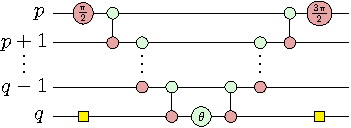
\includegraphics[width=8cm]{figures/zxc/yx_cnot}
% \end{figure}

% Rotation of qubit $p$ into $Y$ basis and rotation of qubit $q$ into $X$ basis, followed rotations back into $Z$ basis at the end of the circuit.

% Left CNOT ladder construction calculates the parity of the qubit state, and applies a rotation in the $Z$ basis if the parity is odd.

% Right CNOT ladder construction to uncompute.

Whilst the second exponential term can be implemented by the phase gadget.
\begin{equation*}
    \text{exp} \left( - i
    \frac{\theta}{2} X_p Y_q \prod_{k=p+1}^{q-1} Z_k \right)
\end{equation*}

% \begin{figure}
% \centering
%     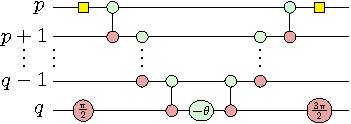
\includegraphics[width=8cm]{figures/zxc/xy_cnot}
% \end{figure}

%%% ----- %%%

Together, they constitute the single-body unitary excitation operator $U^q_p (\theta)$

% \begin{figure}
% \centering
%     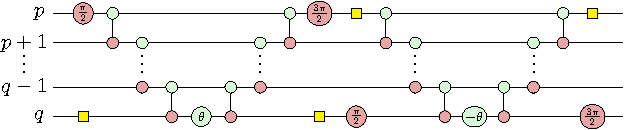
\includegraphics[width=14cm]{figures/zxc/full_cnot}
% \end{figure}

By defining the ordering of spin-orbitals such that adjacent spin-orbitals share the same spatial orbital, adjacent single-body operators commute.

\begin{equation*}
    \left[ \hat\kappa_p^q, \hat\kappa_{p+1}^{q+1} \right] = 0
\end{equation*}\smallskip

The same is therefore true for the resulting qubit operators,

\begin{equation*}
\begin{gathered}
    \left[ F_p^q, F_{p+1}^{q+1} \right] = 0 \\
    p, q \in \text{even} \qquad p+1, q+1 \in \text{odd}
\end{gathered}
\end{equation*}

This allows us to define the parametrised unitary qubit operators in terms of spin-adapted excitation operators.

\begin{equation*}
    U^q_p (\theta) = \text{exp}
    \left[ \theta \left( F_p^q + F_{p+1}^{q+1} \right) \right]
\end{equation*}

In other words, since $F_p^q$ and $F_{p+1}^{q+1}$ commute, we can think of them as a single operator with a single parameter.



% \chapter{\label{phase-gadgets}Phase Gadgets}

\section{Phase Gadgets}
\begin{enumerate}
    \item zx representation
    \item algebraic structure
    \item relation to chemistry
    \item phase gadget decomposition / ladder / bricklayering
\end{enumerate}

\section{Pauli Gadgets}

\section{Commutation Relations}

% \chapter{\label{pauli-gadgets}Pauli Gadgets}


% \chapter{\label{controlled-rotations}Controlled Rotations}

\section{Singly-Controlled Rotations}
Singly-controlled Z rotation.

\begin{figure}[hb]
    \centering
    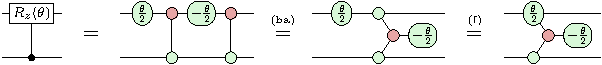
\includegraphics[width=\textwidth]{controlled-rotations/CRZ}
    % \caption{}
    % \label{}
\end{figure}

Singly-controlled X and Y rotations obtained by conjugating the control qubit.

\begin{figure}[hb]
    \centering
    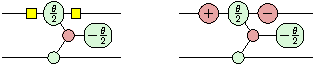
\includegraphics[width=0.6\textwidth]{controlled-rotations/CRX_CRY}
    % \caption{}
    % \label{}
\end{figure}

\section{Doubly-Controlled Rotations}
hello world


\section{Triply-Controlled Rotations}
hello world
hello world

% \chapter{\label{zxfermion-package}ZxFermion Package}

ZxFermion is a Python package built on top of PyZX designed for the manipulation and visualisation of circuits of Pauli gadgets. With built-in Clifford tableau logic using Stim, ZxFermion allows users to quickly implement proofs and test ideas.

VQE algorithms used in quantum chemistry often utilise the UCC framework in which excitation operators have a natural representation as Pauli gadgets. ZxFermion provides a comprehensive toolset designed to be used in a Jupyter notebook environment. Export functionality can be used to generated research paper quality diagrams.

\section{Creating Gadgets}
\section{Creating Circuits of Gadgets}
\section{Pauli \& Clifford Algebra}
\begin{lstlisting}[language=Python]
from zxfermion.gates import X, XPlus, XMinus, Z, ZPlus

XPlus + XMinus
>> Identity
\end{lstlisting}

\section{Architecture-Aware Circuit Extraction}




%%% ========== APPENDICIES  ========== %%%
\startappendices
\subsection{Hadamard}%
\label{appendix-hadamard}

Below are several equivalent definitions of the Hadamard generator. Note that the two rightmost definitions do not require any scalar correction.

\begin{figure}[H]
\centering
    \centering
    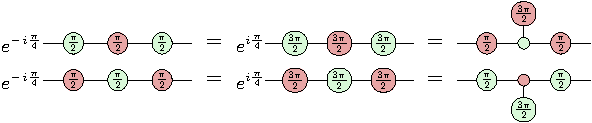
\includegraphics[width=1\textwidth]{chapter-2/hadamard_decomp}
    \caption{Equivalent definitions of the Hadamard generator.}
\end{figure}

%%%

\subsection{Phase Gadgets}%
\label{appendix-phase-gadget-fusion}

We can show how two adjacent phase gadgets fuse using the spider fusion (\ref{spider-fusion}) and bialgebra (\ref{bialgebra}) rules as follows.

\includezxdiagram{chapter-3/phase_gadget_fusion_steps}{0.8}%

%%%

\subsection{Clifford Conjugation Stuff}%
\label{conjugation}

\begin{align*}
    Ce^PC^\dagger &= C \sum_{n=0}^\infty \brac{P^n}{n!} C^\dagger \\
    CP^nC^\dagger &= \sum_{n=0}^\infty \frac{C P^n C^\dagger}{n!} \\
    CP^nC^\dagger &= \sum_{n=0}^\infty \frac{(C P C^\dagger)^n}{n!} \\
    CP^nC^\dagger &= (CPC^\dagger)^n
\end{align*}

%%%

\subsection{CNOT Commutation Relations}

\begin{figure}[H]
    \centering
    \includezxdiagram{chapter-3/cnot_commutations}{1}
    \caption{Complete set of CNOT commutation relations.}
    \label{cnot_commutations}
\end{figure}

\subsection{General One-Body Excitation Operator}%
\label{appendix-one-body-general}

\includezxdiagram{chapter-5/one_body_general_proof}{1}



%%% ========== REFERENCES ========== %%%
\setlength{\baselineskip}{0pt}

{\renewcommand*\MakeUppercase[1]{#1}%
\bibliography{references}{}

\end{document}
